\subsection{地平直行座標への変換}
モーションセンサーから得られる緯度,経度,高度をメートル単位に変換することによって,1回目に取得した位置と2回目に取得した位置からどれくらい移動したのかが分かりやすくなる.そのためには緯度,経度,高度から地平直交座標系に変換する必要がある.地平直行座標への変換の模式図を図\ref{fig:zahyou}に示す.


\begin{figure}[htp]
 \begin{center}
  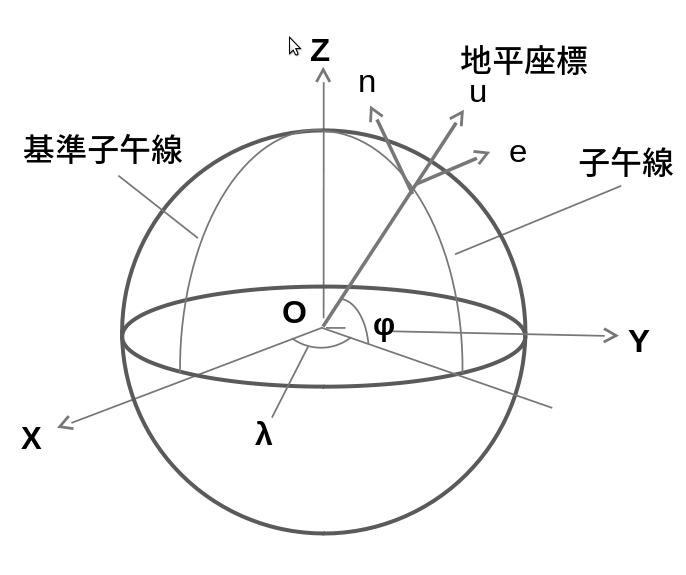
\includegraphics[width=80mm]{img/soft/zahyou.png}
  \caption{地平座標への変換}
  \label{fig:zahyou}%ここに文章中で使用する名前を指定する
 \end{center}
\end{figure}

地平直行座標に変換する際には地球重心を原点とした x y z 座標であるECEF(earth centered, earth fixed)座標に変換する必要がある.
緯度をφ,経度をλ,高度をhとし x y z を求めるために係数Nを求める.
離心率をe,偏平率をfとすると係数Nは式\ref{fig:keisu}によって求めることができる.
\begin{eqnarray}
	N  & = & \frac{a}{\sqrt{1-e^2\sin^2\phi}}
	\label{fig:keisu}
\end{eqnarray}
この係数Nを使用し, x y zそれぞれの座標を求めることができる.
\begin{eqnarray}
	x  & = & (N+h)\cos\phi\cos\lambda
\end{eqnarray}
\begin{eqnarray}
	y  & = & (N+h)\cos\phi\sin\lambda
\end{eqnarray}
\begin{eqnarray}
	z  & = & \{N(1-e^2)+h\}\sin\phi
\end{eqnarray}
上記の式より求めた x y z 座標から地平直行座標に変換する.ECEF直交座標から地平直交座標への変換は,回転と原点移動のみによって実現される.地平座標での位置(e, n, u)は,ECEF直交座標での位置(x, y, z)と原点の位置(x{\scriptsize 0}, y{\scriptsize 0}, z{\scriptsize 0})で,式で求めることができる.
\begin{eqnarray}
  \left(
    \begin{array}{c}
      e\\
      n\\
      u\\ 
    \end{array}
  \right)=R(z,90)R(y,90-\phi)R(z,\lambda)
  \begin{pmatrix}
      x-x_0\\
      y-y_0\\
      z-z_0 
    \end{pmatrix}
\end{eqnarray}

これによって得られた位置(e, n, u)から三平方の定理を用いて距離を算出する.

